\input{style/settings}
\input{style/short_commands}
\pagestyle{fancy}
\fancyhf{}
\fancyhead[R]{página\;\thepage/\pageref{LastPage}}
\fancyhead[L]{Osvaldo Uriel Calderón Dorantes}
\fancyfoot[L]{Imagenología Biomédica}
\fancyfoot[R]{Facultad de Ciencias, UNAM 
\includegraphics[scale=0.13]{style/Sheikah.pdf}}
\fancypagestyle{plain}{
  \fancyfoot[C]{}
}
\makeatletter
\def\@seccntformat#1{%
  \expandafter\ifx\csname c@#1\endcsname\c@section\else
  \csname the#1\endcsname\quad
  \fi}
\makeatother
%%%%%%%%%%%%%%%%%%%%%%%%%%%%%%%%%%%%%%%%%%%%%%%%%%%%%%%
%%%%%%%%%%%%%%%%%%%%%%%%%%%%%%%%%%%%%%%%%%%%%%%%%%%%%%%%%%%
\begin{document}
\begin{flushleft}
Osvaldo Uriel Calderón Dorantes, \hfill Imagenología Biomédica\\
316005171 \hfill osvaldo13576@ciencias.unam  \\
Facultad de Ciencias\\
\underline{Universidad Nacional Autónoma de México}
\end{flushleft}

\begin{flushright}\vspace{-5mm}

\includegraphics[height=1.5cm]{style/logo.pdf}
\end{flushright}
 
\begin{center}\vspace{-1cm}
\textbf{ \large \customfont{Tarea 1\\
Módulo RESONANCIA MAGNÉTICA}}\\
\today
\end{center}
%\medskip\hrule\medskip
%%%%%%%%%%%%%%%%%%%%%%%%%%%%%%%%%%%%%%%%%%%%%%%%
%{\small \textbf{Nota: A las unidades las pondré dentro de corchetes \ec{[\tx{unidad}]} para no confundir entre variables y realizar el análisis dimensional fácilmente.}}
\medskip\hrule\bigskip

\newlength{\strutheight}
\settoheight{\strutheight}{\strut}


A partir del modelo de la distribución de Boltzmann visto en clase, obtenga la relación entre los \textbf{protones} que se encontrarían en un estado de Alta Energía con respecto a los que se encontrarían en un estado de Baja Energía considerando las siguientes condiciones:
\begin{enumerate}[(a)]
  \item Campo magnético de \ec{1.5 \un{T}}, temperatura de \ec{36\un{°C}}.
  \item Campo magnético de \ec{3 \un{T}}, temperatura de \ec{36\un{°C}}
  \item Campo magnético de \ec{7 \un{T}}, temperatura de \ec{36\un{°C}}
\end{enumerate}
Para todos los casos, considere que se tiene un volumen en el que se tienen \ec{3\times10^6} \textbf{protones} orientados de manera paralela y mencione entonces cuántos protones se encontrarían orientados de manera antiparalela.
\bigskip\bigskip



La distribución de Boltzmann está dada por la siguiente relación:
\begin{equation}
  \dfrac{N_\uparrow}{N_\downarrow}=\exp\p{-\dfrac{\Delta E}{kT}}
  \label{eq:distribution}
\end{equation}
donde \ec{N_\uparrow} y \ec{N_\downarrow} son el número de protones en el estado de Alta Energía y Baja Energía respectivamente, \ec{\Delta E} es la diferencia de energía entre los dos estados,  \ec{k} es la constante de Boltzmann y \ec{T} es la temperatura en escala absoluta; observemos que para todos los casos se tiene la misma temperatura,  entonces tenemos que
\ecc{36\un{°C}=309.15 \un{K}}
además:
\begin{equation}
  \Delta E=\gamma\hbar B_0
  \label{eq:e}
\end{equation}
para este caso \ec{\gamma=\gamma_H=42.57 \un{MHz\ec{\cdot}T\ec{^{-1}}}} la constante giromagnética del hidrógeno, \ec{\hbar} es la constante de Planck radial y \ec{B_0} es la intensidad del campo magnético.

Entonces tenemos los valores de las constantes

\dcasos{
\gamma_H=42.57 \un{MHz\ec{\cdot}T\ec{^{-1}}}\\
\hbar=\dfrac{h}{2\pi}=1.055\times10^{-34} \un{J\ec{\cdot}s}\\
T=309.15 \un{K}\\
k=1.381\times10^{-23}\un{J\ec{\cdot}K\ec{^{-1}}}
}
observemos que en la expresión \ec{\dfrac{\Delta E}{kT}=\dfrac{\gamma_H\hbar}{kT}B_0}, \ec{\dfrac{\gamma_H\hbar }{kT}} permanece constante en los tres casos, calculando
\al{\dfrac{\gamma_H\hbar }{kT}&=\dfrac{(42.57 \un{MHz\ec{\cdot}T\ec{^{-1}}})(1.055\times10^{-34} \un{J\ec{\cdot}s})}{(309.15 \un{K})(1.381\times10^{-23}\un{J\ec{\cdot}K\ec{^{-1}}})}\\
&=\dfrac{(42.57\times10^6 \un{s\ec{^{-1}}\ec{\cdot}T\ec{^{-1}}})(1.055\times10^{-34} \un{J\ec{\cdot}s})}{(309.15 \un{K})(1.381\times10^{-23}\un{J\ec{\cdot}K\ec{^{-1}}})}\\
&=\dfrac{(42.57\times10^6 \cancel{\un{s\ec{^{-1}}}})(1.055\times10^{-34} \cancel{\un{J\ec{\cdot}s}})}{(309.15 \cancel{\un{K}})(1.381\times10^{-23}\cancel{\un{J\ec{\cdot}K\ec{^{-1}}}})}\un{T\ec{^{-1}}}\\
&=\dfrac{(42.57\times10^6 )(1.055\times10^{-34} )}{(309.15 )(1.381\times10^{-23})}\un{T\ec{^{-1}}}\\
&=\dfrac{(42.57 )(1.055)}{(309.15 )(1.381)}\times10^{-5}\un{T\ec{^{-1}}}\\
&=1.052\times10^{-6} \un{T\ec{^{-1}}}
}

\pagebreak


\begin{itemize}
  \item \textbf{Campo magnético de \ec{1.5 \un{T}}, temperatura de \ec{36\un{°C}}}:
  
Para este casos tenemos que la intensidad del campo magnético es \ec{B_0=1.5 \un{T}}, por lo que la relación entre el número de protones en el estado de Alta Energía y el de Baja Energía es
\al{\dfrac{N_\uparrow}{N_\downarrow}&=\exp\p{-\dfrac{\gamma_H\hbar}{kT}\cdot B_0}\\
&=\exp\p{-\dfrac{(42.57 )(1.055)}{(309.15 )(1.381)}\times10^{-5}\un{T\ec{^{-1}}}\cdot 1.5\un{T}}\\
&=\exp\p{-\dfrac{(42.57 )(1.055)}{(309.15 )(1.381)}\times10^{-5}\cdot 1.5}\\
&=0.99999842208}
tenemos \ec{3\times10^6} orientados de manera paralela, es decir, \ec{N_\downarrow=3\times10^6} protones de baja energía, por lo tanto tenemos que el número de protones orientados de manera antiparalela son
\al{\dfrac{N_\uparrow}{N_\downarrow}=0.99999842208\implies N_\uparrow&=0.99999842208\times N_\downarrow\\
&=0.99999842208\cdot3\times10^6\\
&=2,999,995.26625}



  \item \textbf{Campo magnético de \ec{3 \un{T}}, temperatura de \ec{36\un{°C}}}:
  

  Para este casos tenemos que la intensidad del campo magnético es \ec{B_0=3 \un{T}}, por lo que la relación entre el número de protones en el estado de Alta Energía y el de Baja Energía es
  \al{\dfrac{N_\uparrow}{N_\downarrow}&=\exp\p{-\dfrac{\gamma_H\hbar}{kT}\cdot B_0}\\
  &=\exp\p{-\dfrac{(42.57 )(1.055)}{(309.15 )(1.381)}\times10^{-5}\un{T\ec{^{-1}}}\cdot 3\un{T}}\\
  &=\exp\p{-\dfrac{(42.57 )(1.055)}{(309.15 )(1.381)}\times10^{-5}\cdot 3}\\
  &=0.9999968442}
  tenemos \ec{3\times10^6} orientados de manera paralela, es decir, \ec{N_\downarrow=3\times10^6} protones de baja energía, por lo tanto tenemos que el número de protones orientados de manera antiparalela son
  \al{\dfrac{N_\uparrow}{N_\downarrow}=0.9999968442\implies N_\uparrow&=0.9999968442\times N_\downarrow\\
  &=0.9999968442\cdot3\times10^6\\
  &=2,999,990.53251}

  \item \textbf{Campo magnético de \ec{7 \un{T}}, temperatura de \ec{36\un{°C}}}:
  Para este casos tenemos que la intensidad del campo magnético es \ec{B_0=7 \un{T}}, por lo que la relación entre el número de protones en el estado de Alta Energía y el de Baja Energía es
  \al{\dfrac{N_\uparrow}{N_\downarrow}&=\exp\p{-\dfrac{\gamma_H\hbar}{kT}\cdot B_0}\\
  &=\exp\p{-\dfrac{(42.57 )(1.055)}{(309.15 )(1.381)}\times10^{-5}\un{T\ec{^{-1}}}\cdot 7\un{T}}\\
  &=\exp\p{-\dfrac{(42.57 )(1.055)}{(309.15 )(1.381)}\times10^{-5}\cdot 7}\\
  &=0.9999926364}
  tenemos \ec{3\times10^6} orientados de manera paralela, es decir, \ec{N_\downarrow=3\times10^6} protones de baja energía, por lo tanto tenemos que el número de protones orientados de manera antiparalela son
  \al{\dfrac{N_\uparrow}{N_\downarrow}=0.9999926364\implies N_\uparrow&=0.9999926364\times N_\downarrow\\
  &=0.9999926364\cdot3\times10^6\\
  &=2,999,977.90923}

  
\pagebreak


\item \textbf{Comparativa}:

\begin{figure}[!ht]
  \center
  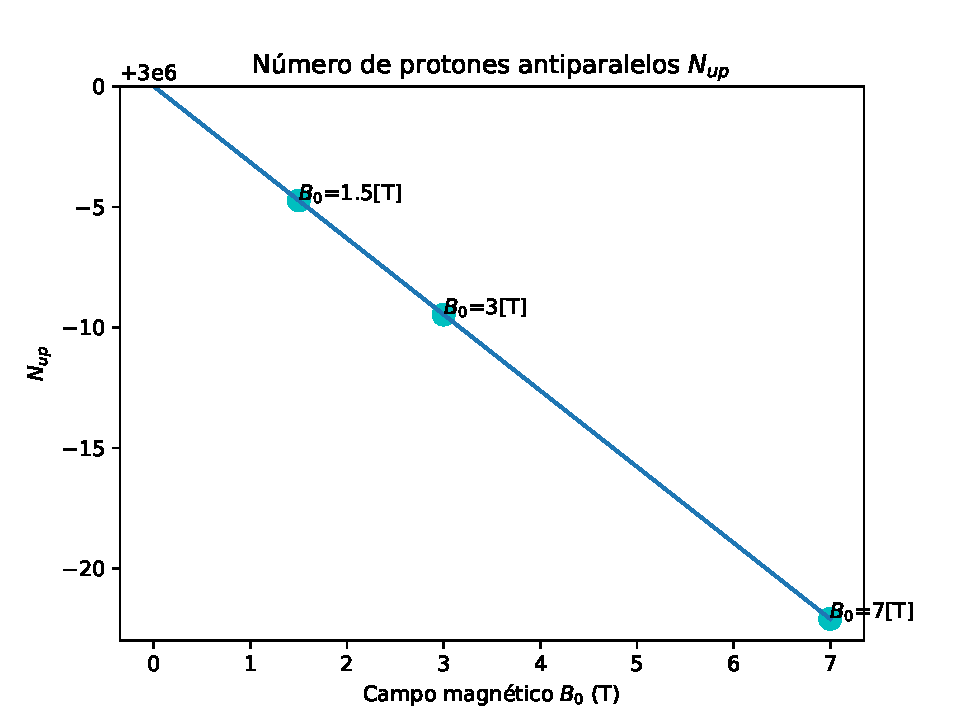
\includegraphics[scale=0.8]{./codes/B0_vs_N_up.pdf}
  \caption{Observamos cómo disminuye los protones alineados de manera antiparalela conforme se aumenta la intensidad del campo magnético.}
  \label{fig:c}
  \end{figure}

\end{itemize}


%\begin{multicols}{2}
%\small{\bibliographystyle{apalike}
%\bibliography{bib}}
%\end{multicols}



%\ftikz{1.5}{figuras/fig.tikz}{}{fig:x}

\end{document}



